\begin{figure}
    \centering
   
    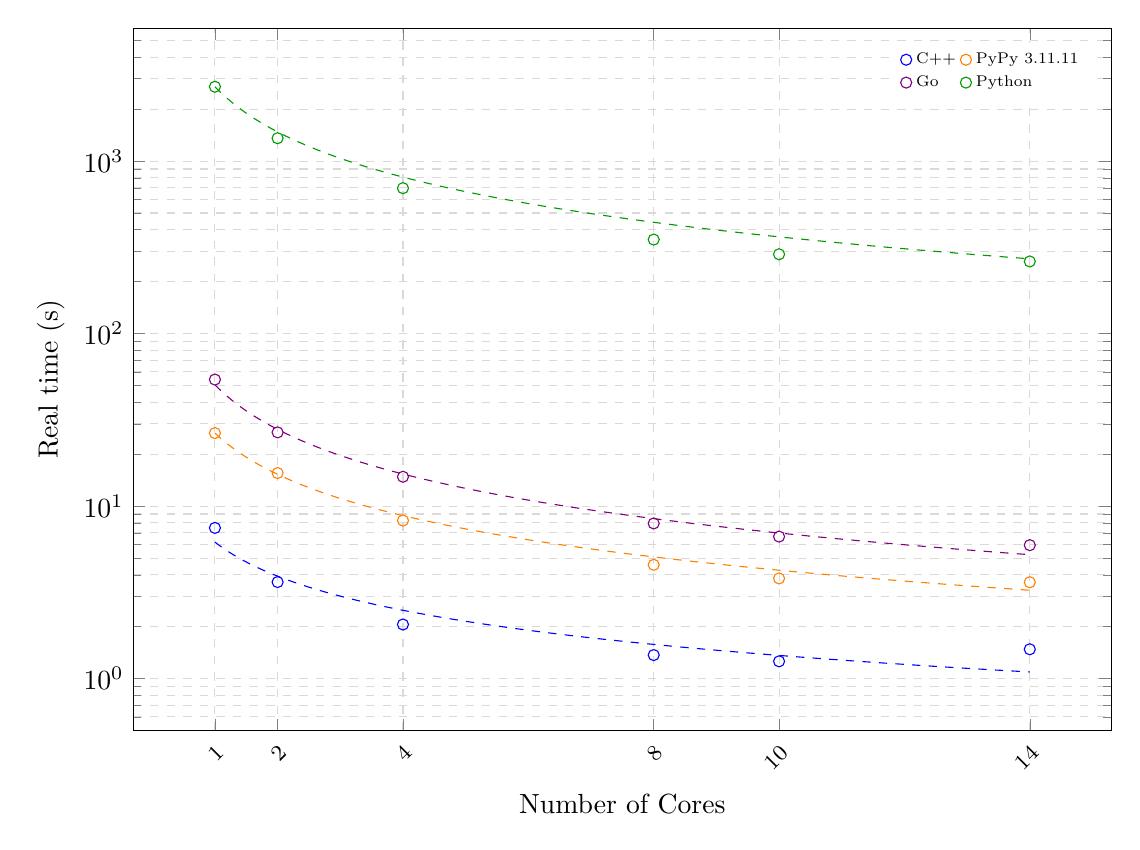
\begin{tikzpicture}
  \begin{semilogyaxis}[
      width=14cm,
      height=10.5cm,
      xlabel={Number of Cores},
      ylabel={Real time (s)},
      ymode=log,
      xmode=linear,
      grid=both,
      minor tick num=1,
      grid style={gray!30,dashed},
      xtick={1,2,4,8,10,14},
      x tick label style={
        font=\footnotesize,
        rotate=45,
        anchor=north east
      },
      legend style={
        at={(0.98,0.98)},
        anchor=north east,
        font=\scriptsize,
        nodes={scale=0.8,transform shape},
        draw=none
      },
      legend columns=2,
      transpose legend,
      legend cell align=left,
    ]
    %% C++ %%
    \addplot[
      blue,
      only marks,
      mark=o,
      mark options={draw=blue,fill=white}
    ]
    table[row sep=\\] {
      x   y     \\
      1   7.48  \\
      2   3.63  \\
      4   2.06  \\
      8   1.37  \\
      10  1.26  \\
      14  1.48  \\
    };
    \addlegendentry{C++}
    % power‐law fit: y = 6.19 * x^(–0.657)
    \addplot[
      blue,
      dashed,
      forget plot,
      domain=1:14,
      samples=200
    ] {6.19 * x^(-0.657)};

    %% Go %%
    \addplot[
      violet,
      only marks,
      mark=o,
      mark options={draw=violet,fill=white}
    ]
    table[row sep=\\] {
      x   y      \\
      1   54.16  \\
      2   26.76  \\
      4   14.80  \\
      8   7.94   \\
      10  6.66   \\
      14  5.94   \\
    };
    \addlegendentry{Go}
    % power‐law fit: y = 50.5 * x^(–0.859)
    \addplot[
      violet,
      dashed,
      forget plot,
      domain=1:14,
      samples=200
    ] {50.5 * x^(-0.859)};

    %% PyPy 3.11.11 %%
    \addplot[
      orange,
      only marks,
      mark=o,
      mark options={draw=orange,fill=white}
    ]
    table[row sep=\\] {
      x   y      \\
      1   26.52  \\
      2   15.55  \\
      4   8.25   \\
      8   4.57   \\
      10  3.81   \\
      14  3.62   \\
    };
    \addlegendentry{PyPy 3.11.11}
    % power‐law fit: y = 26.52 * x^(–0.795)
    \addplot[
      orange,
      dashed,
      forget plot,
      domain=1:14,
      samples=200
    ] {26.52 * x^(-0.795)};

    %% Python %%
    \addplot[
      green!60!black,
      only marks,
      mark=o,
      mark options={draw=green!60!black,fill=white}
    ]
    table[row sep=\\] {
      x    y       \\
      1    2697.08 \\
      2    1356.76 \\
      4    696.75  \\
      8    350.76  \\
      10   288.37  \\
      14   262.00  \\
    };
    \addlegendentry{Python}
    % power‐law fit: y = 2697 * x^(–0.870)
    \addplot[
      green!60!black,
      dashed,
      forget plot,
      domain=1:14,
      samples=200
    ] {2697 * x^(-0.870)};

  \end{semilogyaxis}
\end{tikzpicture}
    \caption{Logarithm Execution time of the mbp example in different programming languages.}
    \label{fig:log-mbp-execution-time}
\end{figure}

\begin{figure}
    \centering
   
    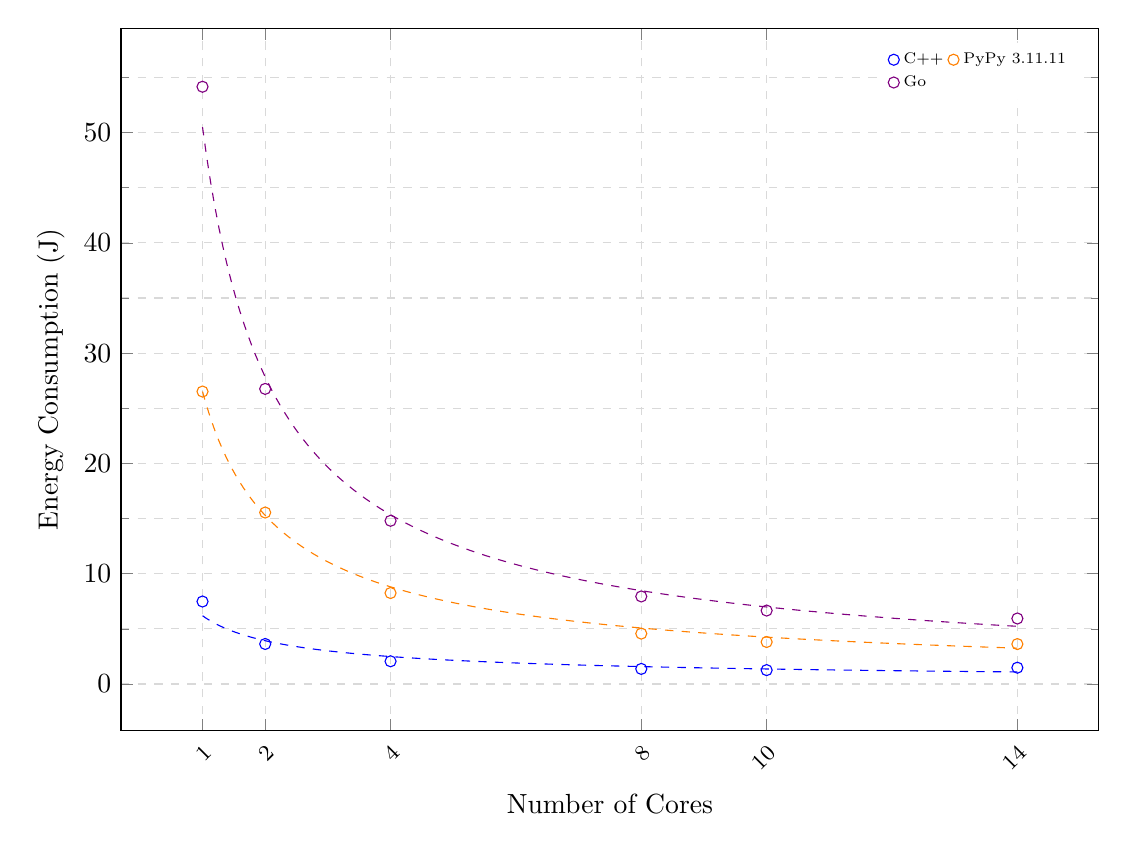
\begin{tikzpicture}
  \begin{axis}[
      width=14cm,
      height=10.5cm,
      xlabel={Number of Cores},
      ylabel={Energy Consumption (J)},
      ymode=linear,
      xmode=linear,
      grid=both,
      minor tick num=1,
      grid style={gray!30,dashed},
      xtick={1,2,4,8,10,14},
      x tick label style={
        font=\footnotesize,
        rotate=45,
        anchor=north east
      },
      legend style={
        at={(0.98,0.98)},
        anchor=north east,
        font=\scriptsize,
        nodes={scale=0.8,transform shape},
        draw=none
      },
      legend columns=2,
      transpose legend,
      legend cell align=left,
    ]
    %% C++ %%
    \addplot[
      blue,
      only marks,
      mark=o,
      mark options={draw=blue,fill=white}
    ]
    table[row sep=\\] {
      x   y     \\
      1   7.48  \\
      2   3.63  \\
      4   2.06  \\
      8   1.37  \\
      10  1.26  \\
      14  1.48  \\
    };
    \addlegendentry{C++}
    % power‐law fit: y = 6.19 * x^(–0.657)
    \addplot[
      blue,
      dashed,
      forget plot,
      domain=1:14,
      samples=200
    ] {6.19 * x^(-0.657)};

    %% Go %%
    \addplot[
      violet,
      only marks,
      mark=o,
      mark options={draw=violet,fill=white}
    ]
    table[row sep=\\] {
      x   y      \\
      1   54.16  \\
      2   26.76  \\
      4   14.80  \\
      8   7.94   \\
      10  6.66   \\
      14  5.94   \\
    };
    \addlegendentry{Go}
    % power‐law fit: y = 50.5 * x^(–0.859)
    \addplot[
      violet,
      dashed,
      forget plot,
      domain=1:14,
      samples=200
    ] {50.5 * x^(-0.859)};

    %% PyPy 3.11.11 %%
    \addplot[
      orange,
      only marks,
      mark=o,
      mark options={draw=orange,fill=white}
    ]
    table[row sep=\\] {
      x   y      \\
      1   26.52  \\
      2   15.55  \\
      4   8.25   \\
      8   4.57   \\
      10  3.81   \\
      14  3.62   \\
    };
    \addlegendentry{PyPy 3.11.11}
    % power‐law fit: y = 26.52 * x^(–0.795)
    \addplot[
      orange,
      dashed,
      forget plot,
      domain=1:14,
      samples=200
    ] {26.52 * x^(-0.795)};

  \end{axis}
\end{tikzpicture}
    \caption{Execution time of the mbp example in different programming languages.}
    \label{fig:linear-mbp-execution-time}
\end{figure}

\begin{table}
    \centering
    \begin{tabular}{lrrrr}
        \hline
        Cores & C++  & Go    & PyPy 3.11.11 & Python    \\
        \hline
        1     & 7.48  & 54.16  & 26.52        & 2,697.08  \\
        2     & 3.63  & 26.76  & 15.55        & 1,356.76  \\
        4     & 2.06  & 14.80  & 8.25         & 696.75    \\
        8     & 1.37  & 7.94   & 4.57         & 350.76    \\
        10    & 1.26  & 6.66   & 3.81         & 288.37    \\
        14    & 1.48  & 5.94   & 3.62         & 262.00    \\
        \hline
    \end{tabular}
    \caption{Execution execution time by implementation and core count}
    \label{tab:mbp-time-execution}
\end{table}